\documentclass[10pt,usenames,dvipsnames]{beamer}
\usepackage{swjtu}
\usepackage[style=apa]{biblatex}
\setbeamertemplate{bibliography item}{\insertbiblabel}
\addbibresource{bibliography.bib}
\usepackage[spanish]{babel}
\usepackage{amsmath} 
\usepackage{amsfonts}
\usepackage{amssymb}
\usepackage{amsthm}
\usepackage{xcolor}
%\usepackage{mdframed}
\usepackage{inputenc}
\usefonttheme{professionalfonts}
%\usefonttheme{serif}
\usepackage{graphicx}
\setbeamercovered{transparent}
\usepackage{ragged2e}
\usepackage{pifont}
\justifying{

\title{\textbf{Evaluating an Agroforestal Intervention in Rural Mexico: Sembrando Vida}}
\subtitle[Semana 3: Análisis de Mociones]{Daniel Kelly}
\author[Daniel Kelly]{El Colegio de México}
%\institute{Asesor: No hay :(}
\date{Septiembre de 2023}

\begin{document}
%% Title page
%% Remove '[plain]' if you need a footline
\begin{frame}[plain]
    \titlepage
\end{frame}

{
\begin{frame}[plain]
    \frametitle{Índice}
    \tableofcontents
\end{frame}
}

\section{Introducción}

\begin{frame}{Introducción}
\textbf{Sembrando Vida} es uno de los \textit{Programas para el Bienestar}, implementados por la Administración Federal 2018-2024 (iniciado en febrero de 2019).
\bigskip
\begin{itemize}
\item El programa consiste en \green{transferencias directas} (\$6.000 mensuales) y \green{apoyos en especie} a \blue{sujetos agrarios} mayores de edad que sean propietarios o posean al menos \orange{2.5 hectáreas} disponibles para trabajar un \textbf{proyecto agroforestal}.
\end{itemize} 
\end{frame}

\begin{frame}
\textbf{Sembrando Vida} está concentrado en promover dos clases principales de proyectos:
\begin{columns}
\begin{column}{0.5\textwidth}
\begin{center}
\textbf{Sistemas Agroforestales}\\
\bigskip
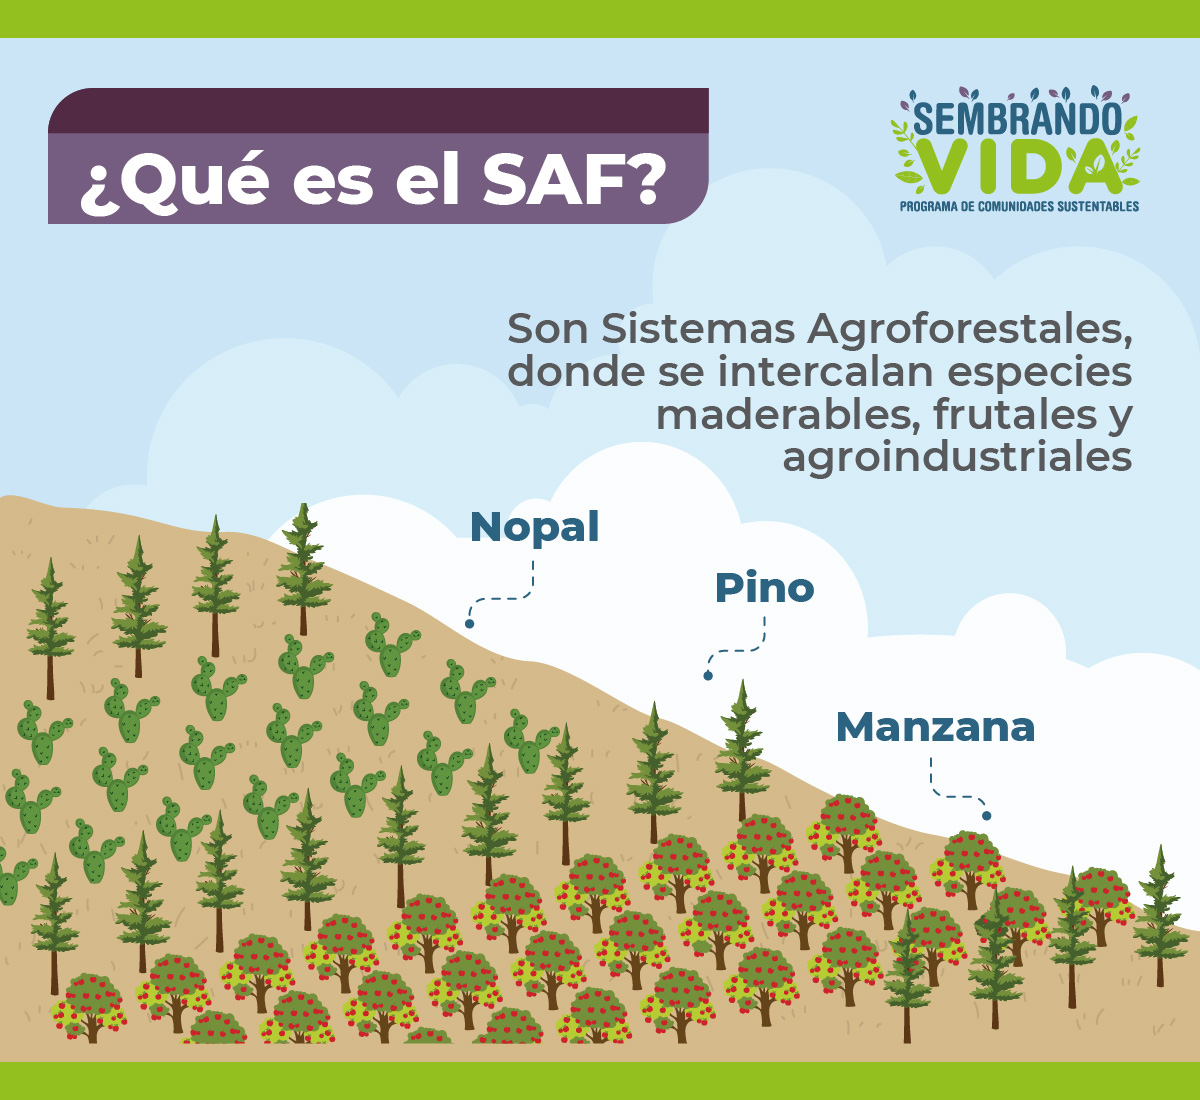
\includegraphics[scale=.12]{Gráficas/SAF.jpeg} 
\end{center}
\end{column}
\begin{column}{0.5\textwidth}
\begin{center}
\textbf{Milpa Intercalada con Arboles Frutales}\\
\bigskip
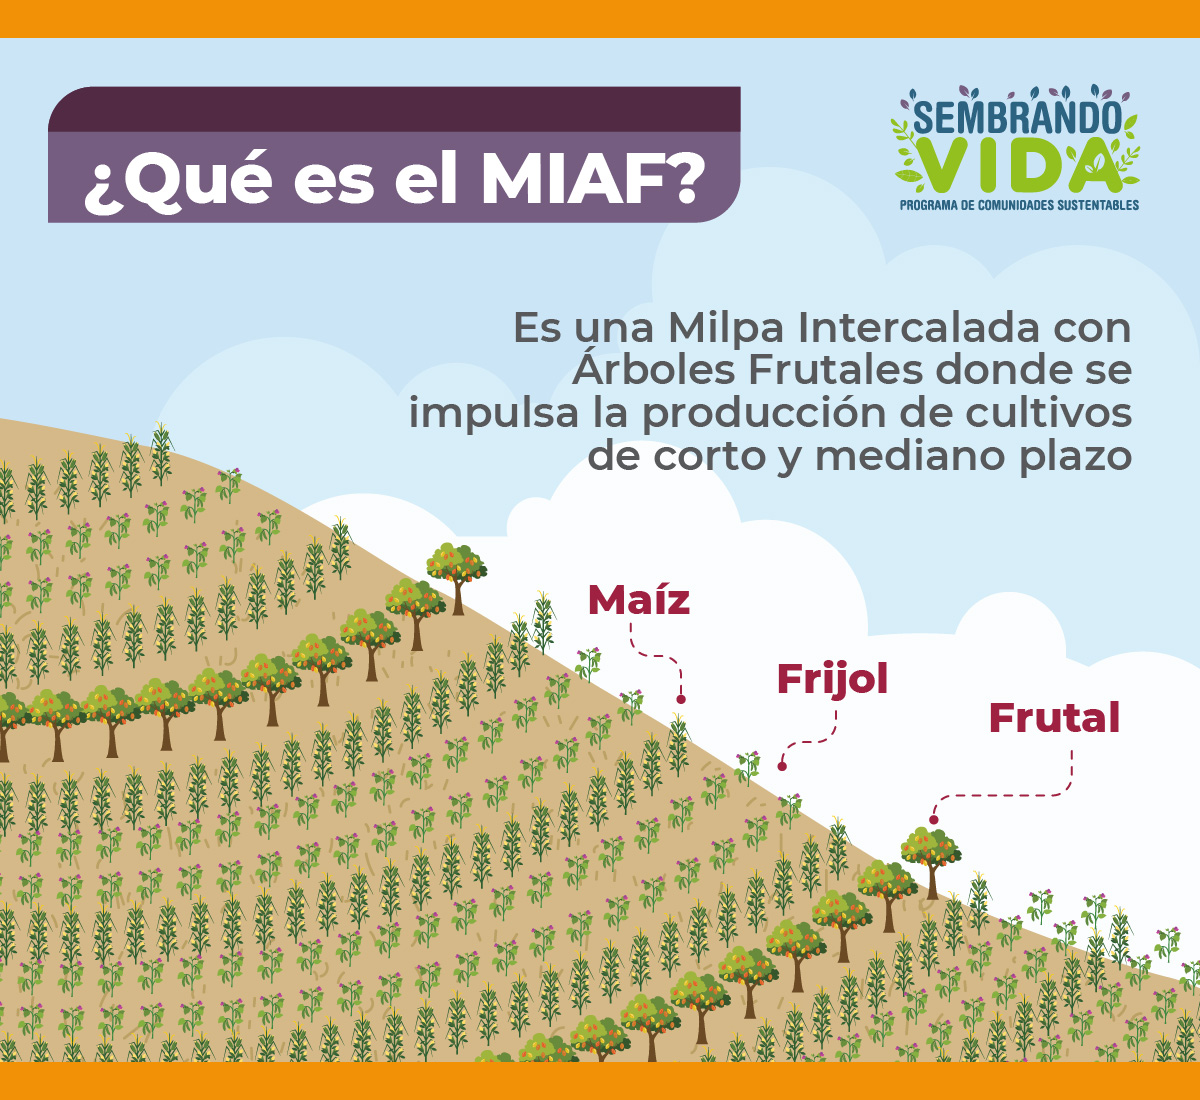
\includegraphics[scale=.12]{Gráficas/MIAF.jpeg} 
\end{center}
\end{column}
\end{columns}
\end{frame}

\begin{frame}
De acuerdo con el Gobierno Federal\footnote{\href{https://www.gob.mx/bienestar/acciones-y-programas/programa-sembrando-vida}{\color{blue}{Programa Sembrando Vida}}}, los objetivos del programa son: (1) Rescate del campo mexicano; (2) Regeneración del tejido social; (3) Reactivar las economías locales.\\
\bigskip
Para 2023, el Gobierno Federal reporta \footnote{\href{https://programasparaelbienestar.gob.mx/wp-content/uploads/2023/05/4.-30052023-STP-Programas-del-Bienestar.pdf}{\color{blue}{Avance de los Programas para el Bienestar 2023}}}:
\begin{itemize}
\item \blue{37 mil millones de pesos} invertidos en el programa en 2023.
\item \blue{449,686} empleos permanentes en \blue{21} estados. 
\item \blue{1,124,215} hectáreas en el programa.
\item \blue{1,411 millones} de arboles plantados (en parcelas y viveros).
\end{itemize}
\end{frame}

\section{Pregunta de Investigación}

\begin{frame}{Preguntas de Investigación}
\textbf{\alert{1.}} ¿El programa Sembrando Vida tiene efectos sobre la \blue{productividad/eficiencia} del campo mexicano?\\
\bigskip
\ding{228} \indent{[\green{\cite{castle}}] encuentra efectos significativos y positivos sobre la productividad del campo en los lugares estudiados (\textit{(...) positive impact on yield (...)}).}\\
\bigskip
\ding{228} \indent{[\green{\cite{amadu}}] identifica que el principal mecanismo de acción a través del cual la política agroforestal afecta la productividad general del campo es mediante el aumento en la fertilidad del suelo (mayores nutrientes y otros beneficios medioambientales).}\\
\bigskip
\ding{228} \indent{[\green{\cite{felix}}] sostiene que el crecimiento poblacional en las zonas rurales impone presiones adicionales que evitan la práctica de la agricultura de subsistencia. Las intervenciones agroforestales pueden recuperar el suelo y contribuir a romper este ciclo.
}
\end{frame}

\begin{frame}
\ding{228} \indent{[\green{\cite{coulibaly}}] encuentra efectos positivos y estadísticamente significativos sobre la seguridad alimentaria de las familias pertenecientes a comunidades rurales (parece que en el corto plazo, puede superarse la agricultura de subsistencia).}\\
\bigskip
\ding{228} \indent{[\green{\cite{dai}}] encuentra efectos positivos y estadísticamente significativos sobre el ingreso de pequeños hogares rurales a partir de programas de \textit{intercropping}.}\\
\end{frame}

\begin{frame}
\textbf{\alert{2.}} ¿Están estos efectos diferenciados por el \blue{régimen de propiedad de la tierra} imperante en un municipio?\\
\bigskip
\textbf{Obstáculos:}
\begin{itemize}
    \item Debilidad del entorno institucional.
    \item Posibilidad de distintas relaciones de cooperación entre campesinos de acuerdo con el régimen de propiedad de la tierra imperante.
\end{itemize}
\bigskip
El Gobierno Federal reporta \blue{8,917 ejidos} registrados en el programa. Aunque estos no se pueden seguir directamente en los datos, si se puede identificar los municipios en dónde predominan.
\end{frame}


\section{Contribución a la Literatura}

\begin{frame}{Contribución a la Literatura}
Este trabajo pretende establecer una relación causal entre la implementación del programa \textbf{Sembrando Vida}. Contribuímos a la literatura existente en 3 principales respectos:\\
\bigskip
\begin{enumerate}
\pause
\item Identificar \textbf{efectos diferenciados} según la estructura productiva de los distintos municipios. En otras palabras, identificar si los municipios en dónde impera la propiedad social (ejido) poseen un mayor/menor efecto causal como respuesta al programa.
\bigskip
\pause
\item Identificar si los beneficios en \textbf{productividad} o \textbf{eficiencia} obtenidos a partir de la intervención compensan la inversión realizada por el Gobierno Federal en la ejecución del programa.
\end{enumerate}
\end{frame}

\begin{frame}
\begin{enumerate}
\pause
\item \textbf{(Posiblemente)} Tratar de identificar efectos sobre el bienestar de los individuos. La literatura existente tiene un gran enfoque en los efectos sobre precios de alimentos y seguridad alimentaria. \pause $\to$ Problema: Datos que nos permitan el seguimiento de estas variables.
\end{enumerate}
\bigskip

\end{frame}



\section{Estrategia de Identificación}

\subsection{Datos}

\begin{frame}{Datos}
Los datos usados para la estimación provienen de \orange{tres fuentes} principales:\\
\bigskip
\begin{enumerate}
\item Sistema de Información Agroalimentaria y Pesquera: Anuario Estadístico de la Producción Agrícola.
\bigskip
\item Registro Único de Beneficiarios: Sembrando Vida.
\bigskip
\item Registro Nacional Agrario: Catálogo de Núcleos Agrarios.
\end{enumerate}
\end{frame}

\begin{frame}{Anuario Estadístico de la Producción Agrícola}
Estadísticas proporcionadas por la \green{Secretaría de Agricultura y Desarrollo Rural} a través del \green{Sistema de Información Agroalimentaria y Pesquera}.\\
\bigskip
\begin{itemize}
\item Contiene información \orange{anual} a \orange{nivel municipal} de la producción agrícola, específicamente, reporta 3 estadísticas:
\begin{enumerate}
\item Superficie Total Sembrada.
\item Superficie Total Cultivada.
\item Valor Total de la Producción.
\end{enumerate}
\bigskip
\item Esto nos permite identificar nuestras dos variables de interés por municipio:
\begin{enumerate}
\item \textbf{Eficiencia de la Producción}: Porción sembrada que efectivamente se cosecha.
\item \textbf{Productividad}: Valor promedio de cada hectárea.
\end{enumerate}
\end{itemize}
\end{frame}

\begin{frame}{Registro Único de Beneficiarios}
Información proporcionada directamente por el \green{Gobierno Federal}, que contiene la base de datos completa de beneficiarios del programa \textbf{Sembrando Vida}.\\
\bigskip
Contiene información \orange{bimestral} a \orange{nivel individual} de cada beneficiario, en particular:
\begin{itemize}
\item Localización Geográfica: Entidad y Municipio en dónde se localiza el beneficiario.
\item Monto recibido mensualmente por el beneficiario.
\item Edad del beneficiario.
\item Fecha de inscripción al programa.
\end{itemize}
\end{frame}

\begin{frame}
\begin{center}
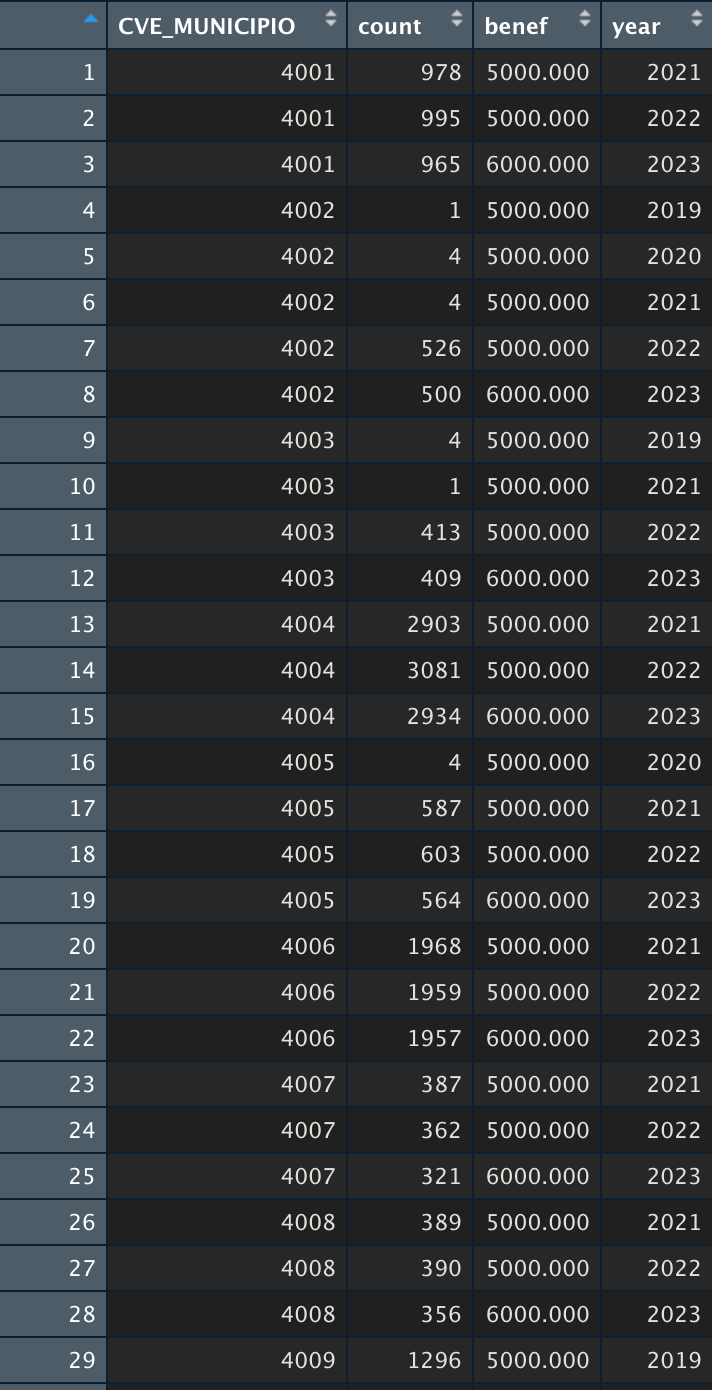
\includegraphics[scale=0.35]{Gráficas/Base de Datos.png} 
\end{center}
\end{frame}

\begin{frame}{Registro Agrario Nacional (RAN)}
El \green{Catálogo de Núcleos Agrarios} del \green{Registro Agrario Nacional} contiene el listado completo de núcleos agrarios en el país (particularmente nos interesa la propiedad ejidal).\\
\bigskip
\begin{itemize}
\item Esto nos permite identificar los municipios en dónde la estructura de propiedad social es más persistente. 
\end{itemize}
\end{frame}

\begin{frame}{Base de Datos Final}
En conjunto, tenemos una base de datos con observaciones \orange{anuales} (desde 2010) a \orange{nivel municipio} que contiene:
\begin{itemize}
\item Valor, superficie sembrada y superficie cosechada de la producción agrícola.
\item Medida de penetración del programa \textbf{Sembrando Vida} en el municipio (a partir del número de beneficiarios).
\item Medida de la estructura de la propiedad social en el municipio* (a partir del número de entradas en el Registro Agrario Nacional).
\item Una serie de controles a nivel municipal:
\begin{itemize}
\item Población.
\item Tamaño del Municipio.
\item Precios de los Productos Agrícolas*. 
\end{itemize}
\end{itemize}
\end{frame}


\subsection{Técnica de Estimación}

\begin{frame}{Estimación}
\begin{itemize}
\item \textbf{Grupo de Tratamiento:} Todos los municipios en condición de \orange{rezago social} en dónde el programa sembrando vida está presente (que cuentan con \blue{beneficiarios activos} en el patrón) \footnote{Podría ser conveniente establecer un requerimiento de la clase ''con más de $X$ años en el programa''.}.
\item \textbf{Grupo de Control:} Todos los municipios rurales en condición de rezago social en el país.
\end{itemize}
\bigskip
La \textbf{heterogeneidad} en la aplicación del programa (21 de 32 estados de la república) nos permite explotar la máxima variación posible. Igualmente, la base a nivel individual nos permite no solo construir una \textit{dummy} que indique la pertenencia al tratamiento, sino determinar la \textbf{intensidad} del tratamiento.
\end{frame}

\begin{frame}
El modelo a estimar (\textit{preeliminar}) está dado por:\\
\bigskip
\begin{equation}
Y_{it} = \delta_0 + \mathbf{\alpha_1} \mathbf{w_t} + \mathbf{\alpha_2} \mathbf{T_i} + \beta (\mathbf{w_t} \cdot \mathbf{T_i}) + \gamma \mathbf{X_{it}} + \varepsilon_{it}
\end{equation}
Dónde:\\
\bigskip
\begin{itemize}
\item $\mathbf{w_t}$ indica si la observación pertenece al periodo previo o posterior al tratamiento.
\item $\mathbf{T_i}$ es una variable (continua) que indica el número de beneficiarios en cada municipio (por cada 100,000 habitantes).
\item $\mathbf{X_{it}}$ es un vector de controles (población por municipio, territorio, \green{ingreso}, etc.).
\end{itemize}
\end{frame}

\section{Siguientes Pasos}

\begin{frame}{Siguientes Pasos}
\begin{itemize}
\item Concluir con el \textit{matching} de las bases de datos.
\bigskip
\item Proceder a la estimación empírica: 
\begin{itemize}
\item Es probable que se incluyan \textit{lagged-effects}, haciendo énfasis en que el efecto de la intervención puede tardar más de un periodo en manifestarse.
\item Pruebas de robustez: Intentar identificar efectos diferenciados según el tipo de cultivo (\textit{perenne} o \textit{cíclicos}).
\end{itemize}
\bigskip
\item Analizar resultados y proceder a la fase de redacción.
\end{itemize}

\end{frame}

%% Final page
\begin{frame}[plain]
    \begin{picture}(0,0)
        \put(-21.5, -164){
\includegraphics[width=\paperwidth]{Imágenes/final_page_bg.png}}
    \end{picture}
\end{frame}


%% Bibliography
\appendix
\begin{frame}[allowframebreaks]{Referencias}
    \printbibliography
\end{frame}
\end{document}}
